\documentclass{beamer} 
\usepackage{beamerthemeTUM}
\usepackage[latin1]{inputenc} 
\usepackage{amsmath} 
\usepackage{amsfonts} 
\usepackage{amssymb} 
\usepackage{algorithm} 
\usepackage{algorithmicx} 
\usepackage[noend]{algpseudocode}
\usepackage{multicol} 
\usepackage{url}
\usepackage{graphics}
\usepackage{multicol}
\usepackage{eso-pic}
\usepackage{pst-node}
\usepackage{xcolor}
\usepackage{multido}
\usepackage{subfigure}
\usepackage{pstricks}
\usepackage{float} 
\usepackage{graphicx}

\graphicspath{{figures/}}

\setlang{en}


\author{Sebastian Lehnerer} 
\title{Feature and Label Selection for \\Multi Label Learning} 
\email{lehnerer@in.tum.de}
\date{\today}
\institute[2011]{Technische Universit\"at M\"unchen}


\begin{document} 


\AddToShipoutPicture{\TitlePicture}
\maketitle
%\frame{\titlepage}
\ClearShipoutPicture
\AddToShipoutPicture{\BackgroundPicture}
\AtBeginPart{\frame{\partpage}}


\frame{
	\frametitle{Multi-Label Learning}
	\begin{itemize}
		\item find a bipartionen of given labels into positive and negative sets (relevant/irrelevant)
		\item example
			\begin{itemize}
				\item instance $ I = \{X_{1}...X_{n} \cup Y_{1},Y_{2},Y_{3},Y_{4},Y_{5}\} $ where feature attributes are $X$ and target (label) attributes are noted as $Y$.
				\item aim is to produce a bipartionen $ P_I := \{Y_1,Y_3\}, N_I := \{Y_2,Y_4,Y_5\} $ which classifies labels $ Y_1, Y_3 $ as positive, the rest negative.
			\end{itemize}
	\end{itemize}
}

\frame{
	\frametitle{Multi-Label Learning}
	\begin{center}
		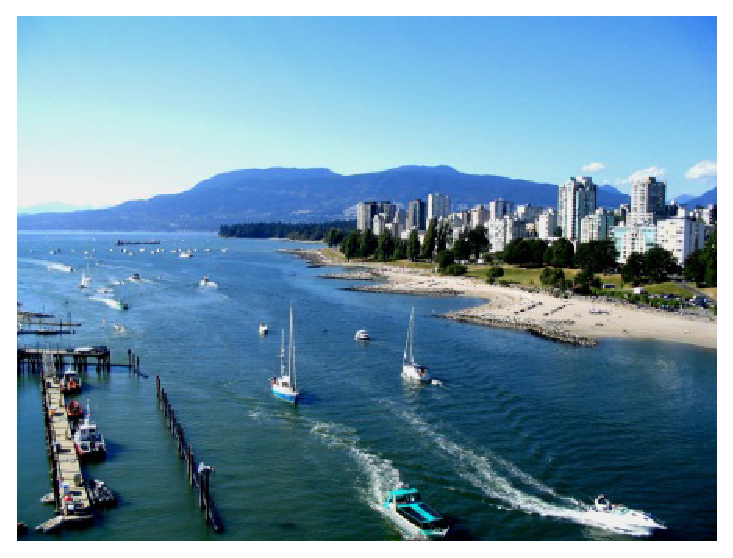
\includegraphics[scale=.5]{figures/Vancouver-skyline.eps} 	
	\end{center}
	\begin{itemize}
		\item labelset \begin{small} $ Y := \{forest, desert, city, island, beach, hills, boat\} $\end{small} 
		\item bipartion \begin{small} $ P := \{city, beach, hills, boat\}, N := \{forest, desert, island\} $\end{small} 
	\end{itemize}
}

\frame{
	\frametitle{Feature and Label Selection for \\Multi Label Learning}
	\begin{itemize}
		\item multi-label datasets can be huge and contain a lot of information for different labels.
		\item labels don't need to overlap, eg. attribute $ X_1 $ is useless to $ Y_1 $ but determining for $ Y_2 $
		\item \emph{multi-label datasets may contain subsets of features and labels which are highly relevant intrinsically with lower relation to the rest of the data}
	\end{itemize}
}

\frame {
	\frametitle{Feature and Label Selection for \\Multi Label Learning}
	\begin{figure}
		\begin{center}
		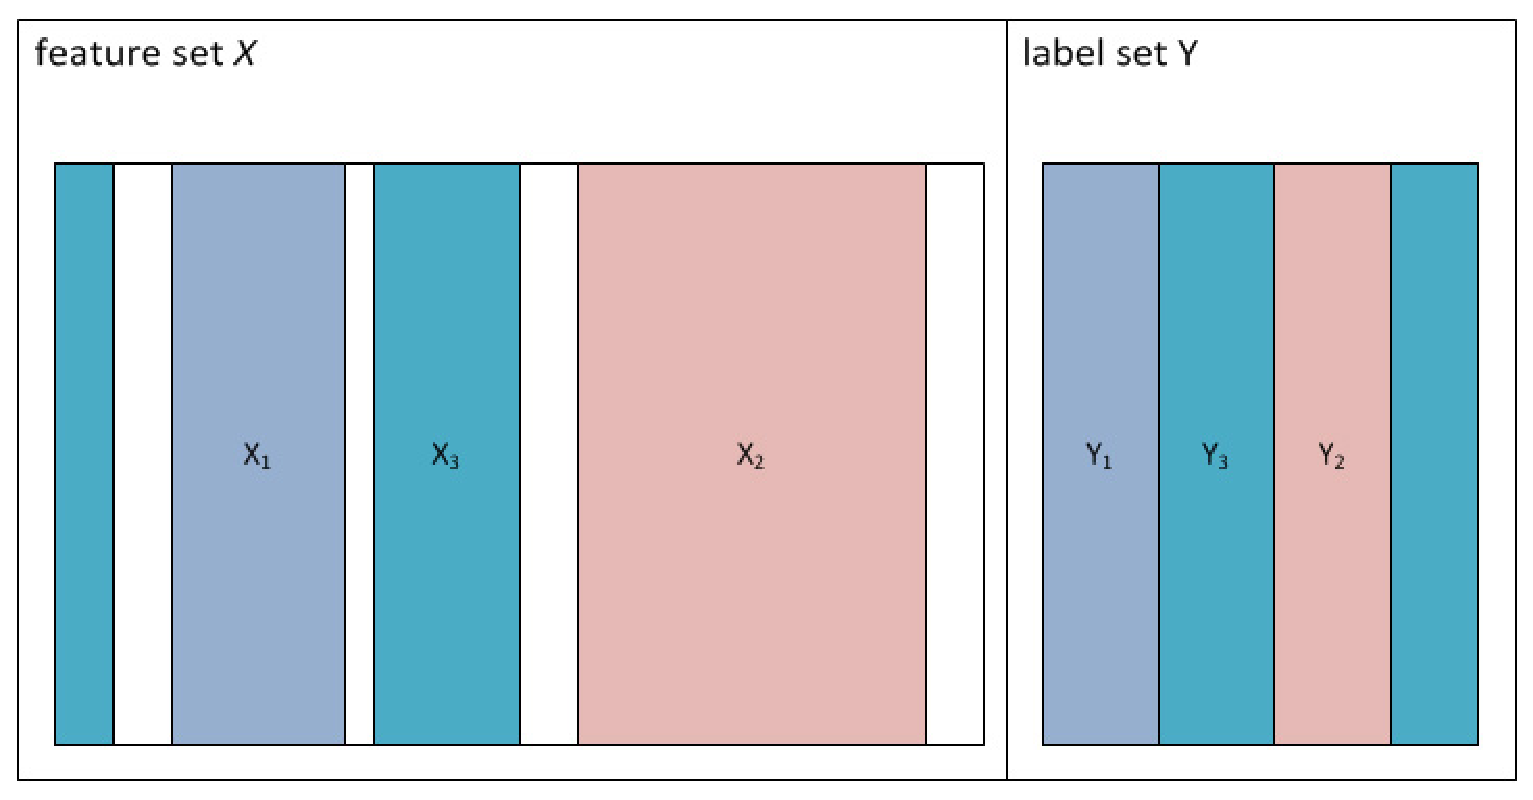
\includegraphics[scale=.35]{figures/featurelabelset.eps}
		\caption{split of a multi-label dataset in different subsets where the featureset $ X_i $ belongs to the labelset $ Y_i $.}	
		\end{center}
	\end{figure}
}

\frame {
	\frametitle{Feature and Label Selection for \\Multi Label Learning}
	\begin{itemize}
		\item aim of this work is to find and evaluate those subsets.
		\item three different methods are developed and tested:
			\begin{itemize}
				\item FCML (feature score based clustering)
				\item TCML (tanimoto distance based clustering)
				\item CML (instance based clustering)
			\end{itemize}
	\end{itemize}
}

\frame{
\frametitle{CML}
 \begin{itemize} 
  \item using transposed dataset, each attribute will become an instance
  \item clustering over those instances
  \item clusters resolve directly into groups by splitting into labels and features
 \end{itemize}
}


\frame{
 {\insertsection} 
		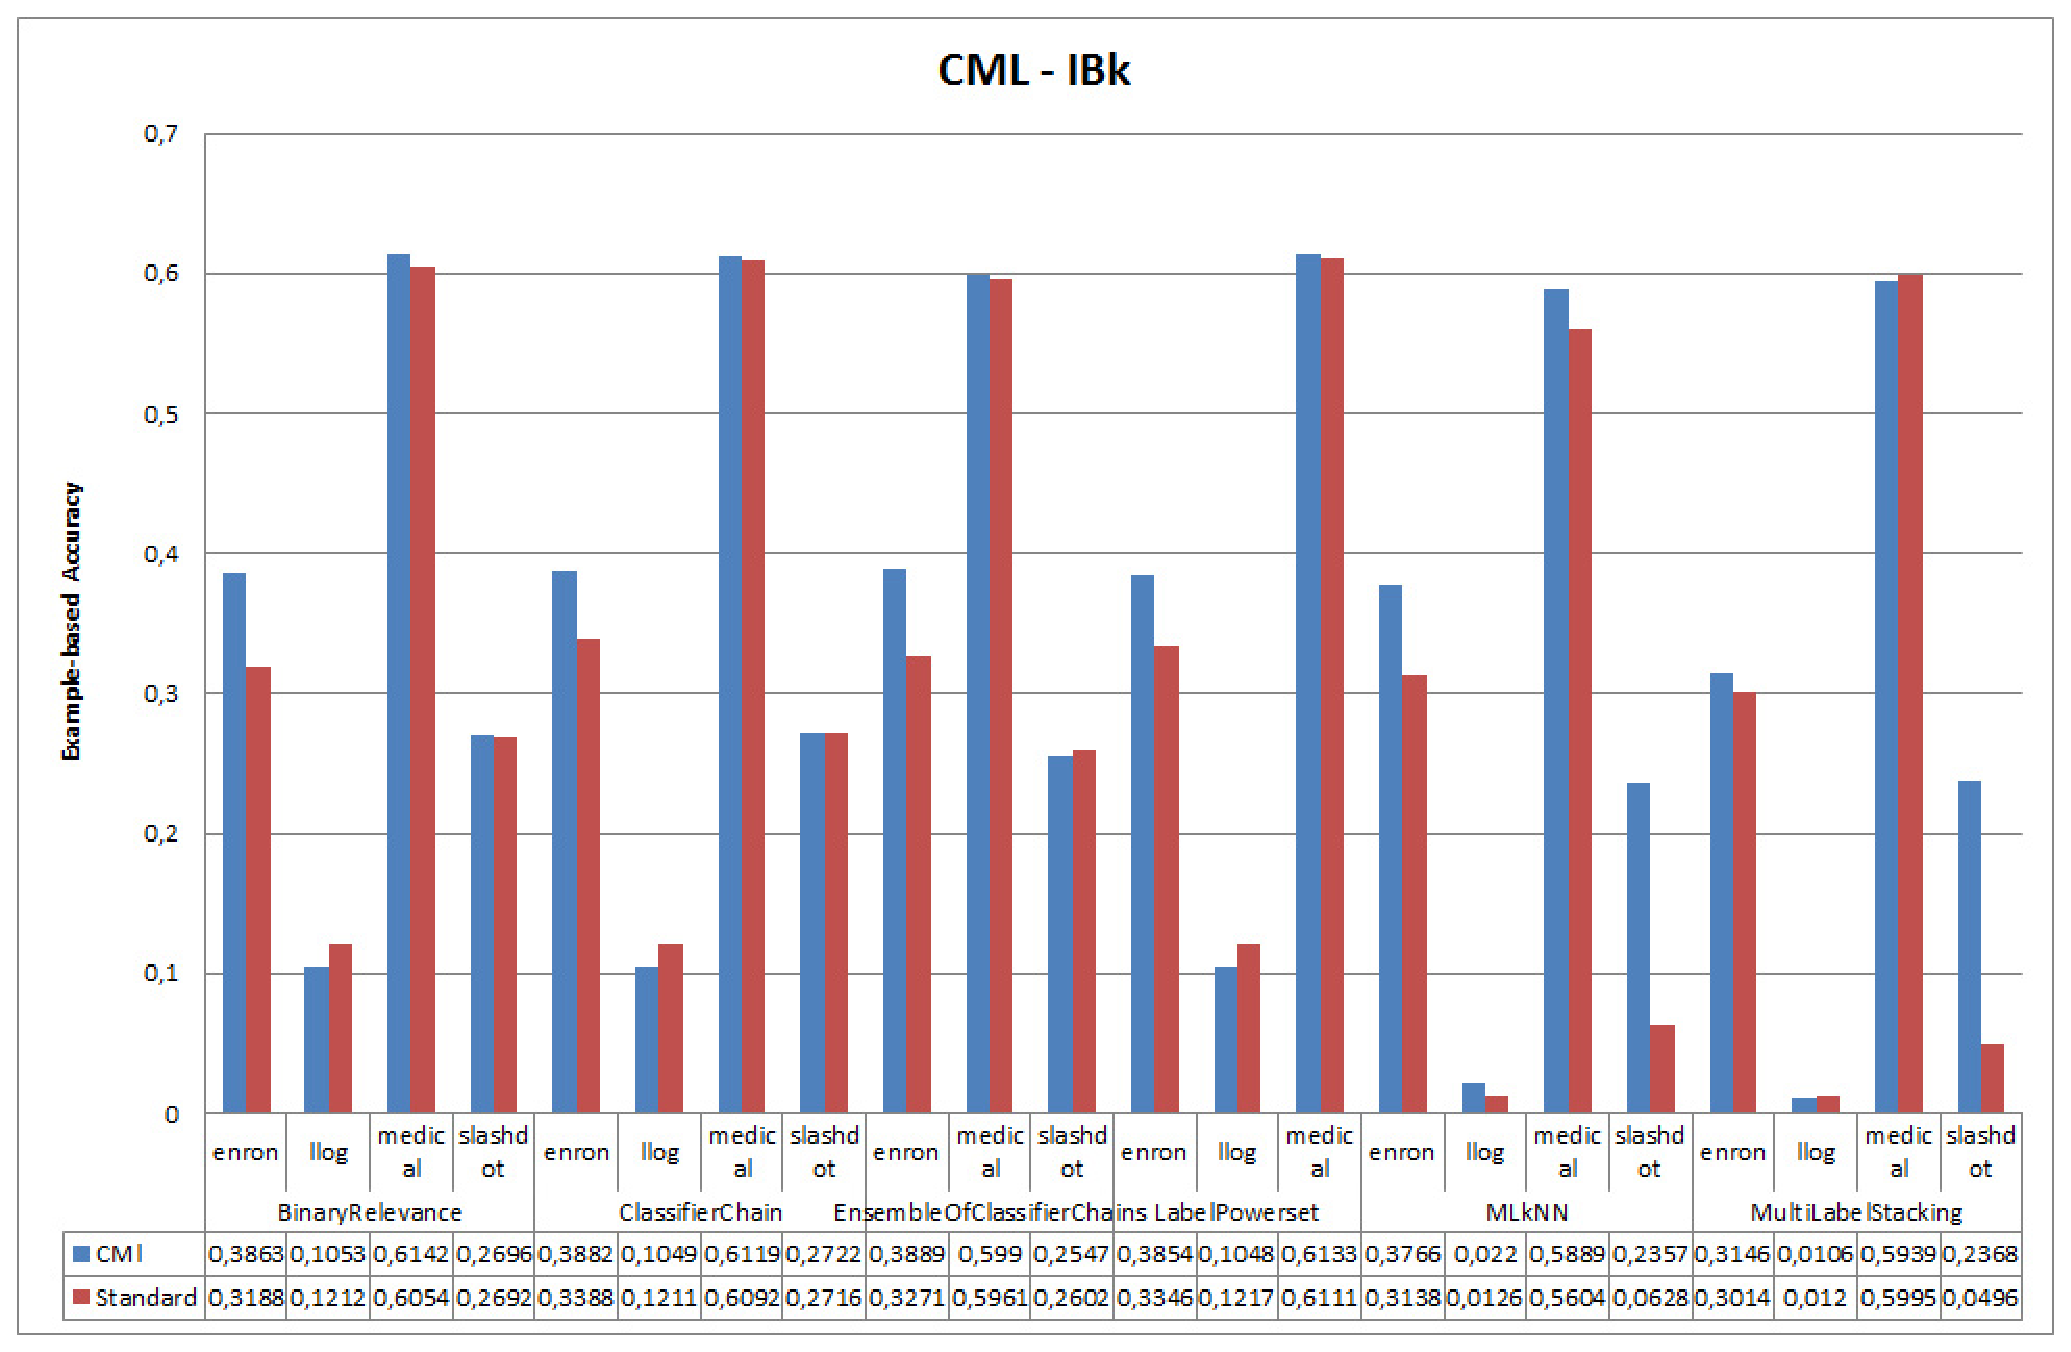
\includegraphics[scale=.3]{figures/cml_results_ibk.eps} 
}


\frame{
 {\insertsection} 
		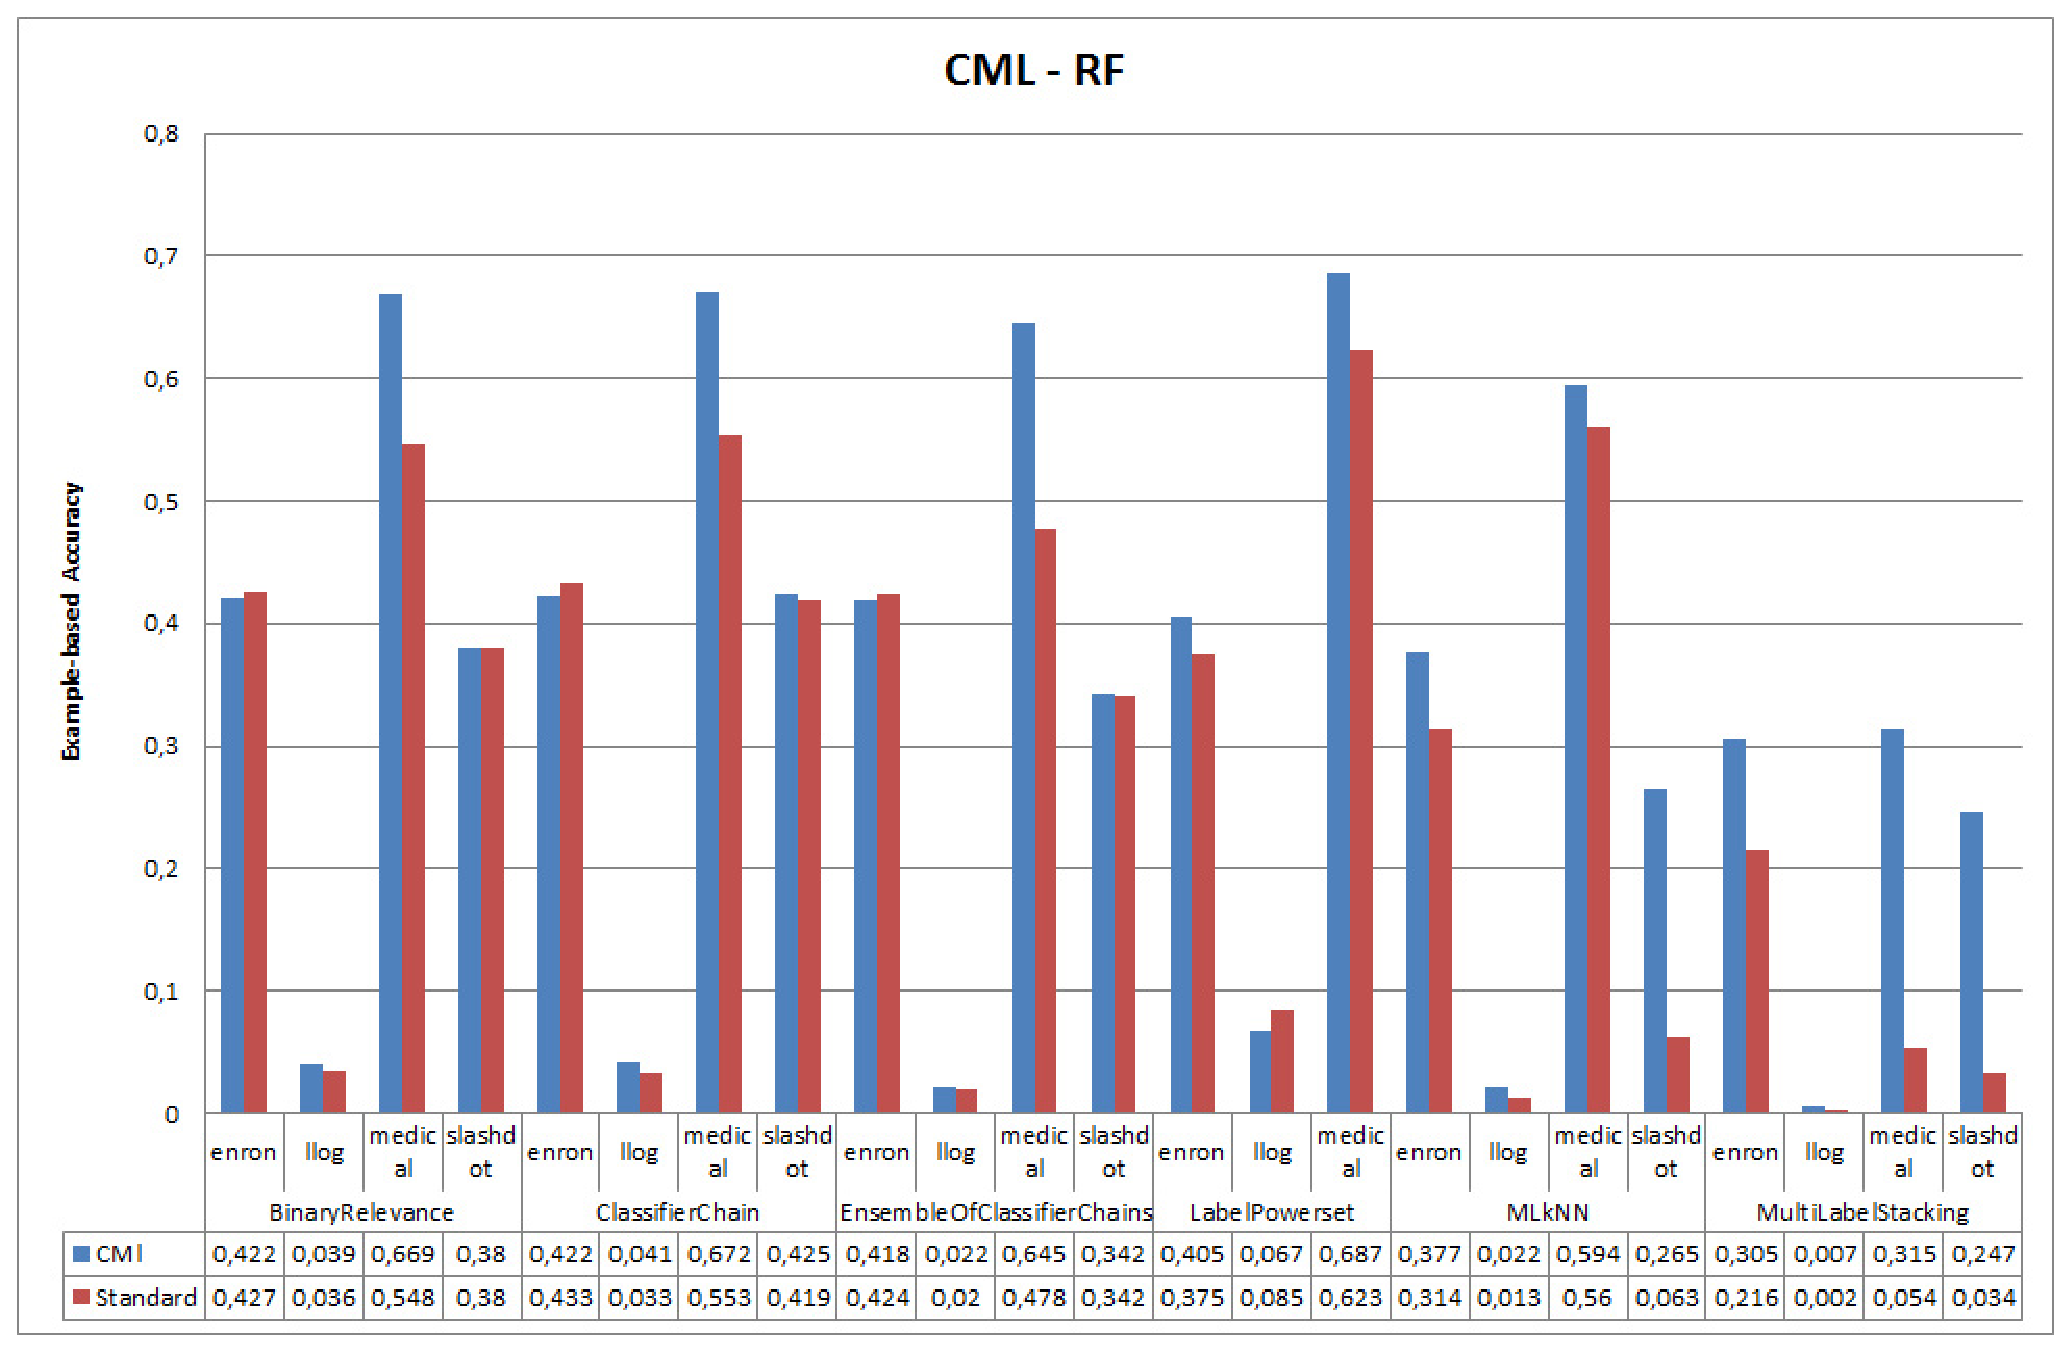
\includegraphics[scale=.3]{figures/cml_results_rf.eps} 
}


\frame{
 {\insertsection} 
		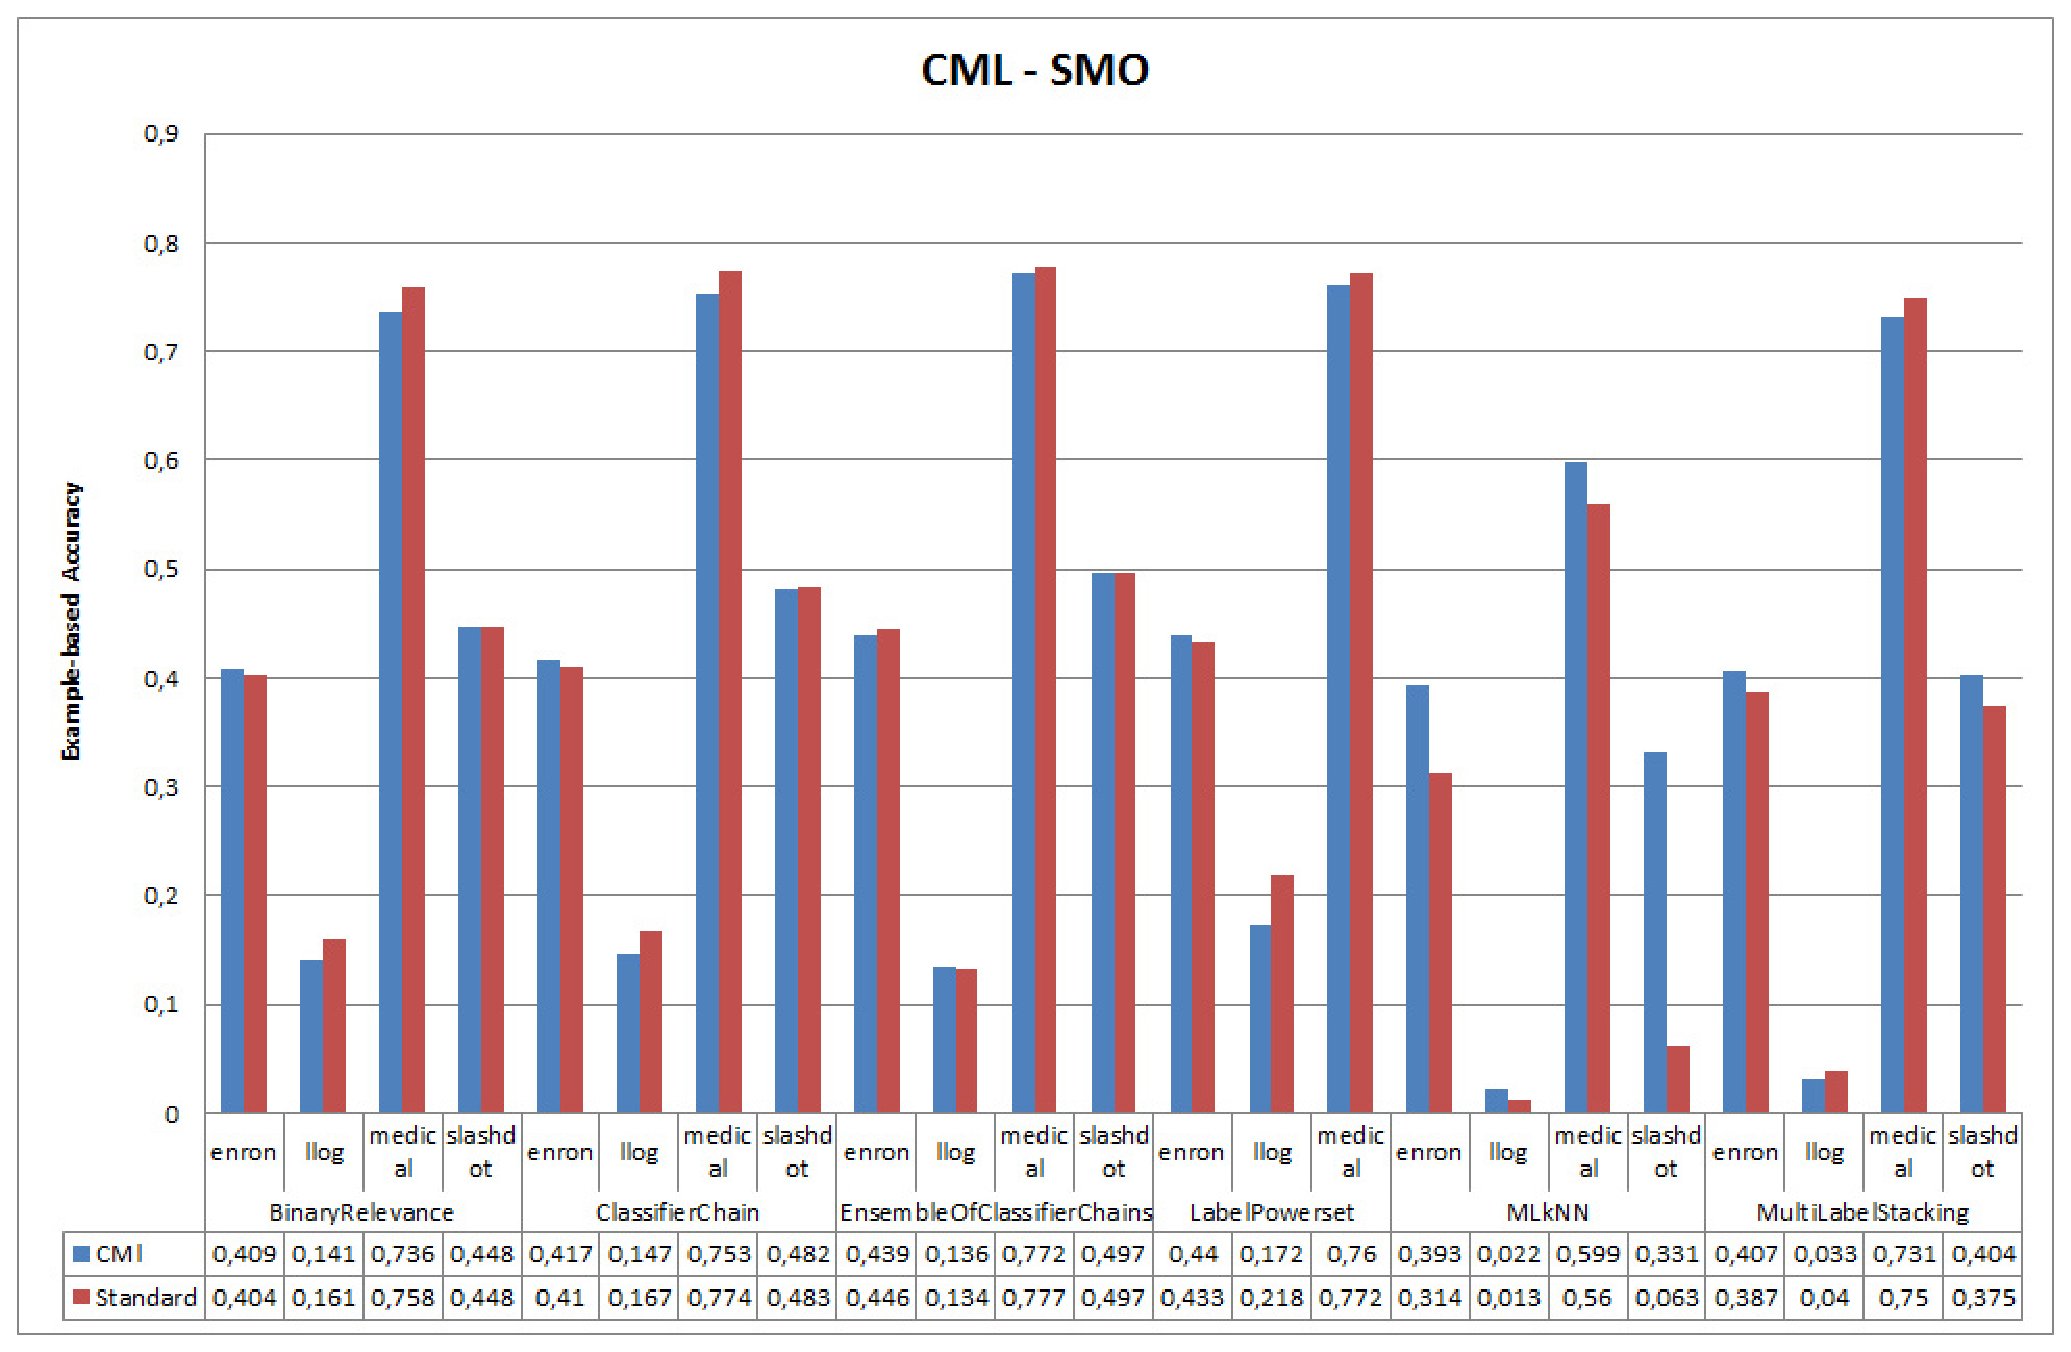
\includegraphics[scale=.3]{figures/cml_results_smo.eps} 
}

\frame{
	{\insertsection}
	example cluster characteristics (\(\varnothing\) over folds)
	\scriptsize {
	\begin{itemize}
		\item enron\\
		\(\varnothing\) number of clusters : 8\\
		\(\varnothing\) number of cluster ($> 2$ labels) : 2\\
		\(\varnothing\) number of labels per cluster: 13.3	
		\item llog\\
		\(\varnothing\) number of clusters : 4\\
		\(\varnothing\) number of cluster ($> 2$ labels) : 4\\
		\(\varnothing\) number of labels per cluster: 37.5	
		\item medical\\
		\(\varnothing\) number of clusters : 8.4\\
		\(\varnothing\) number of cluster ($> 2$ labels) : 2\\
		\(\varnothing\) number of labels per cluster: 10.7	
		\item slashdot\\
		\(\varnothing\) number of clusters : 10\\
		\(\varnothing\) number of cluster ($> 2$ labels) : 2\\
		\(\varnothing\) number of labels per cluster: 4.4	
	\end{itemize}
	}
}

\frame{
\frametitle{TCML}
 \begin{itemize} 
  \item feature selection for every label, where other labels are
    treated as normal features
    \end{itemize} 
    \begin{eqnarray*} 
      Y_{1} &\leftarrow & \{X_{1}...X_{n} \cup Y_{2}...Y_{n}|X_{i},Y_{i}\in\{0,1\}\}\\ 
      Y_{2} &\leftarrow & \{X_{1}...X_{n} \cup Y_{1},Y_{3}...Y_{n}|X_{i},Y_{i}\in\{0,1\}\}\\ 
      &\vdots &\\ 
      Y_{n} &\leftarrow & \{X_{1}...X_{n} \cup Y_{1}...Y_{n-1}|X_{i},Y_{i}\in\{0,1\}\} 
    \end{eqnarray*} 
  
}

\frame{
 \frametitle{TCML}
  \begin{itemize}
  	\item using label feature sets as vectors $ <0,1,0,0,1,0,\cdots,1,0> $      
  	\item Hierachical Clustering using the Tanimoto Distance.
  	\begin{equation*}
		T_s(X,Y) =  \frac{\sum_i ( X_i \land Y_i)}{\sum_i ( X_i \lor Y_i)}
	\end{equation*}
  	\item Single, Complete, Average and Mean Clustering
  	\item no. of clusters: $2,4,6$
  \end{itemize} 
}

\frame{
 {\insertsection} 
		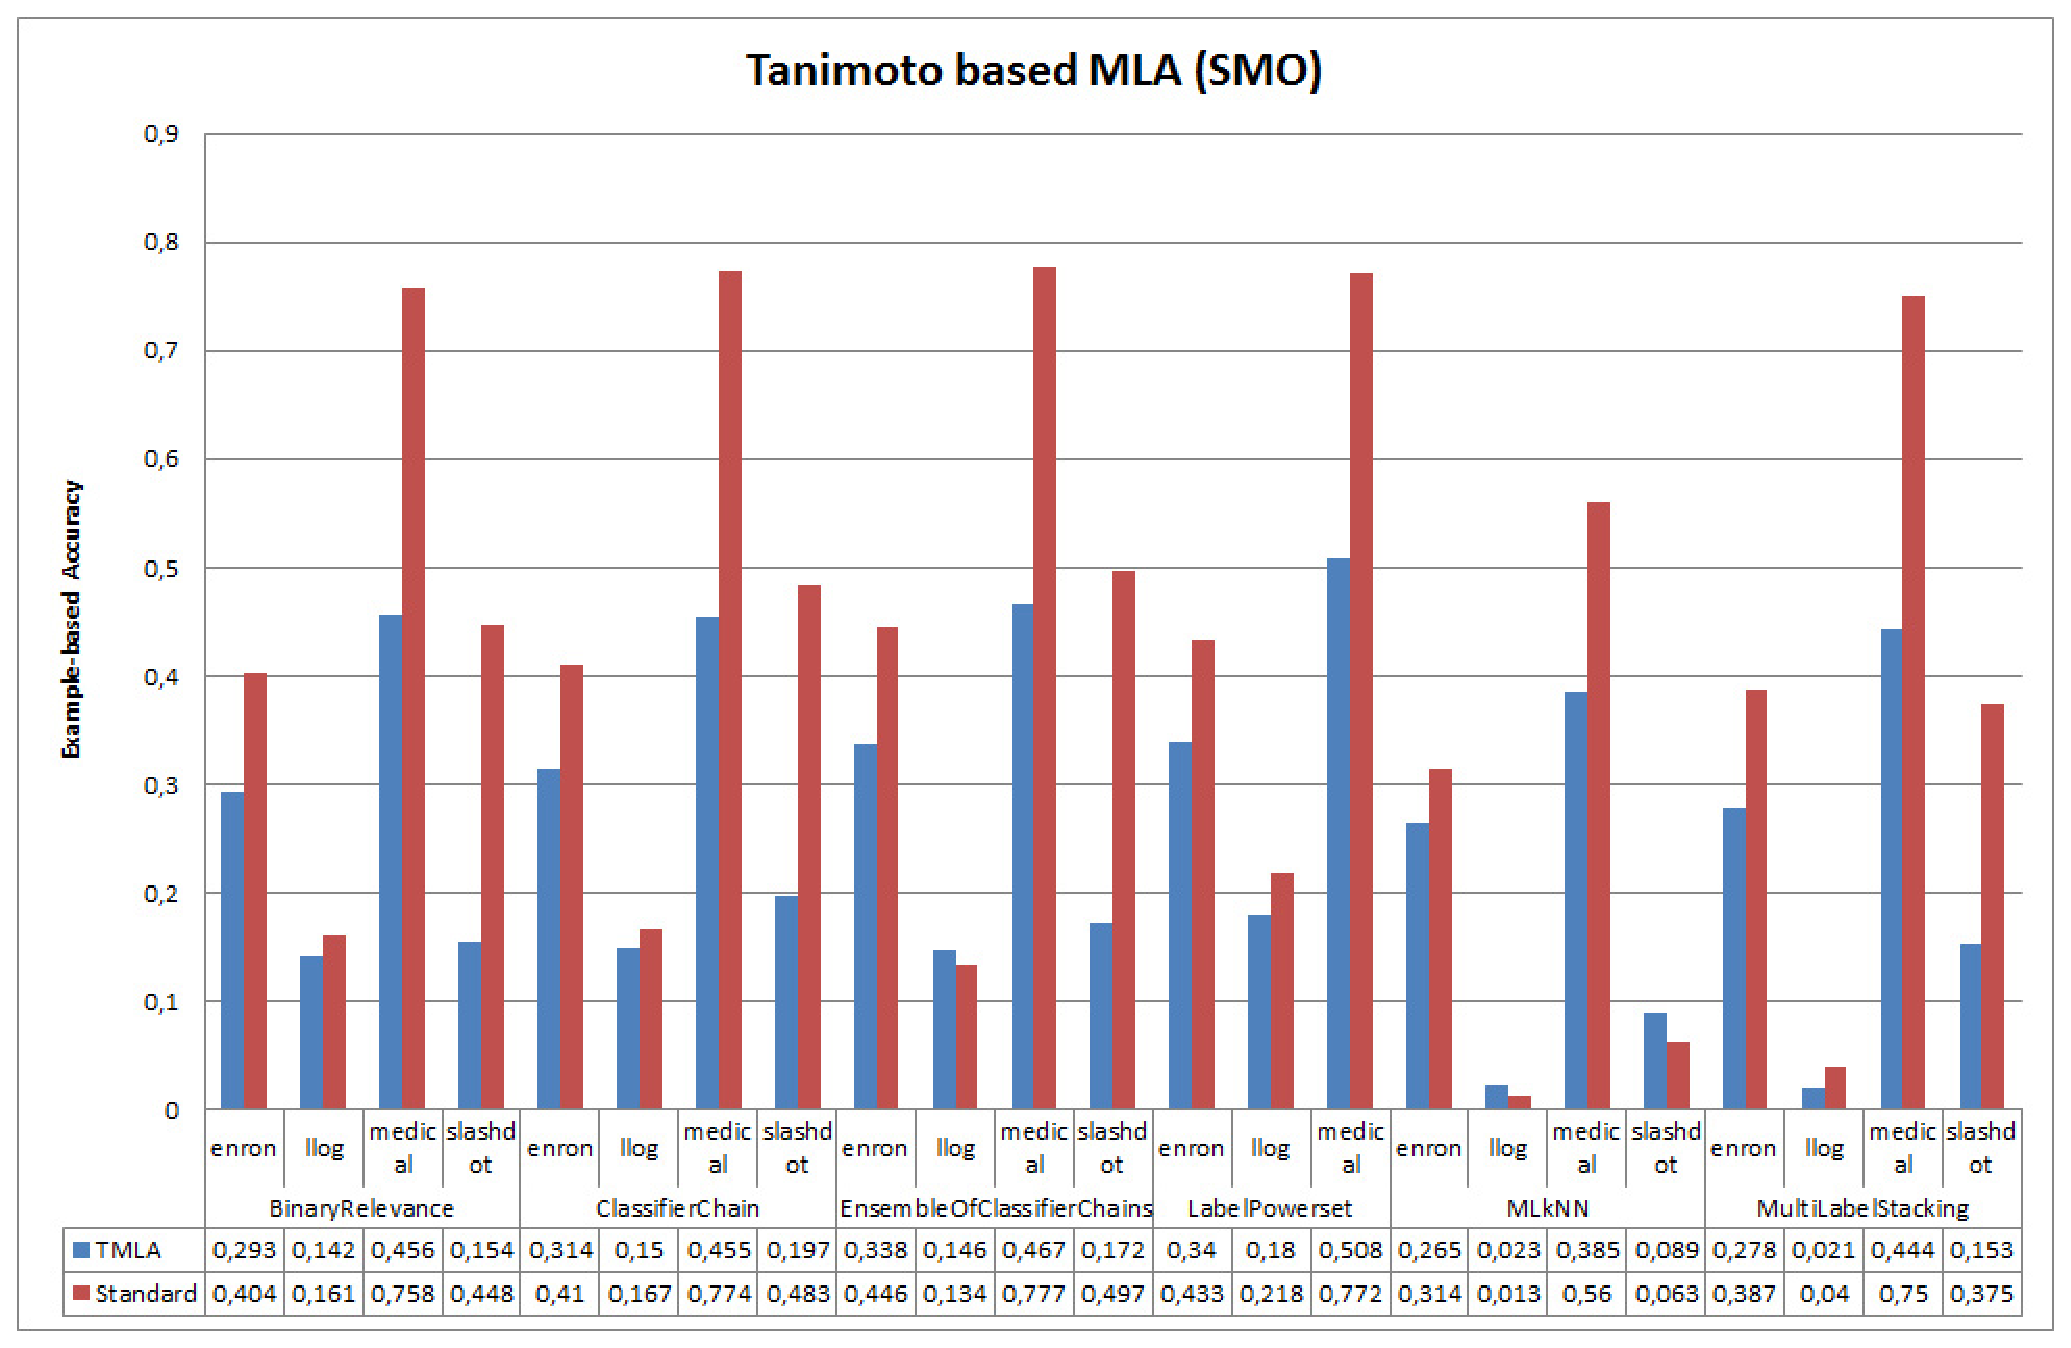
\includegraphics[scale=.3]{figures/tmla_results_smo.eps}
}

\frame{
 {\insertsection} 
		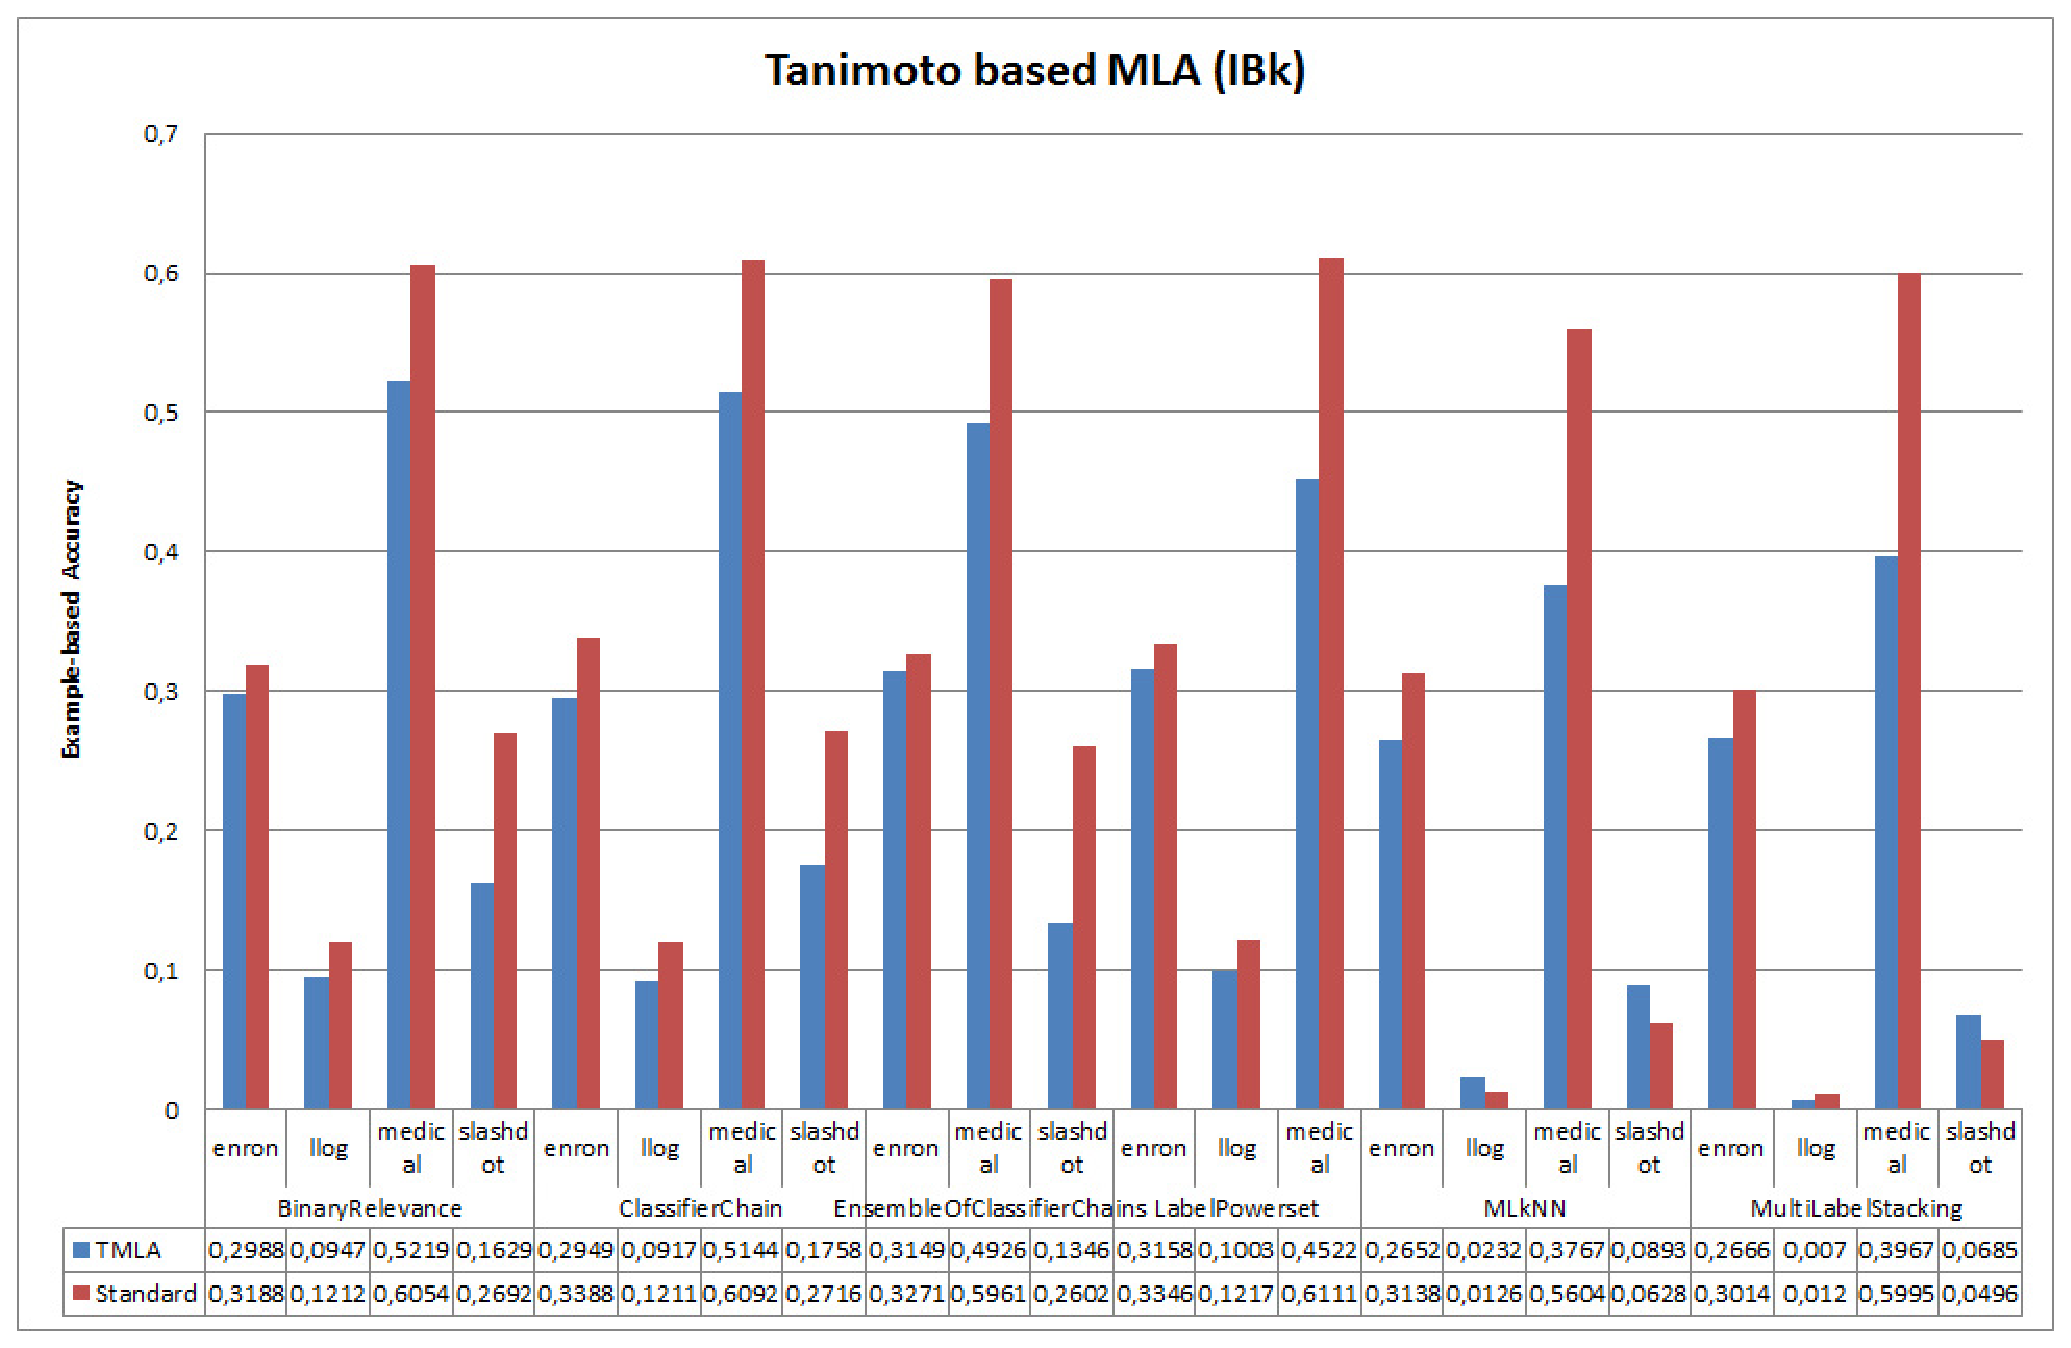
\includegraphics[scale=.3]{figures/tmla_results_ibk.eps}
}

\frame{
 {\insertsection} 
		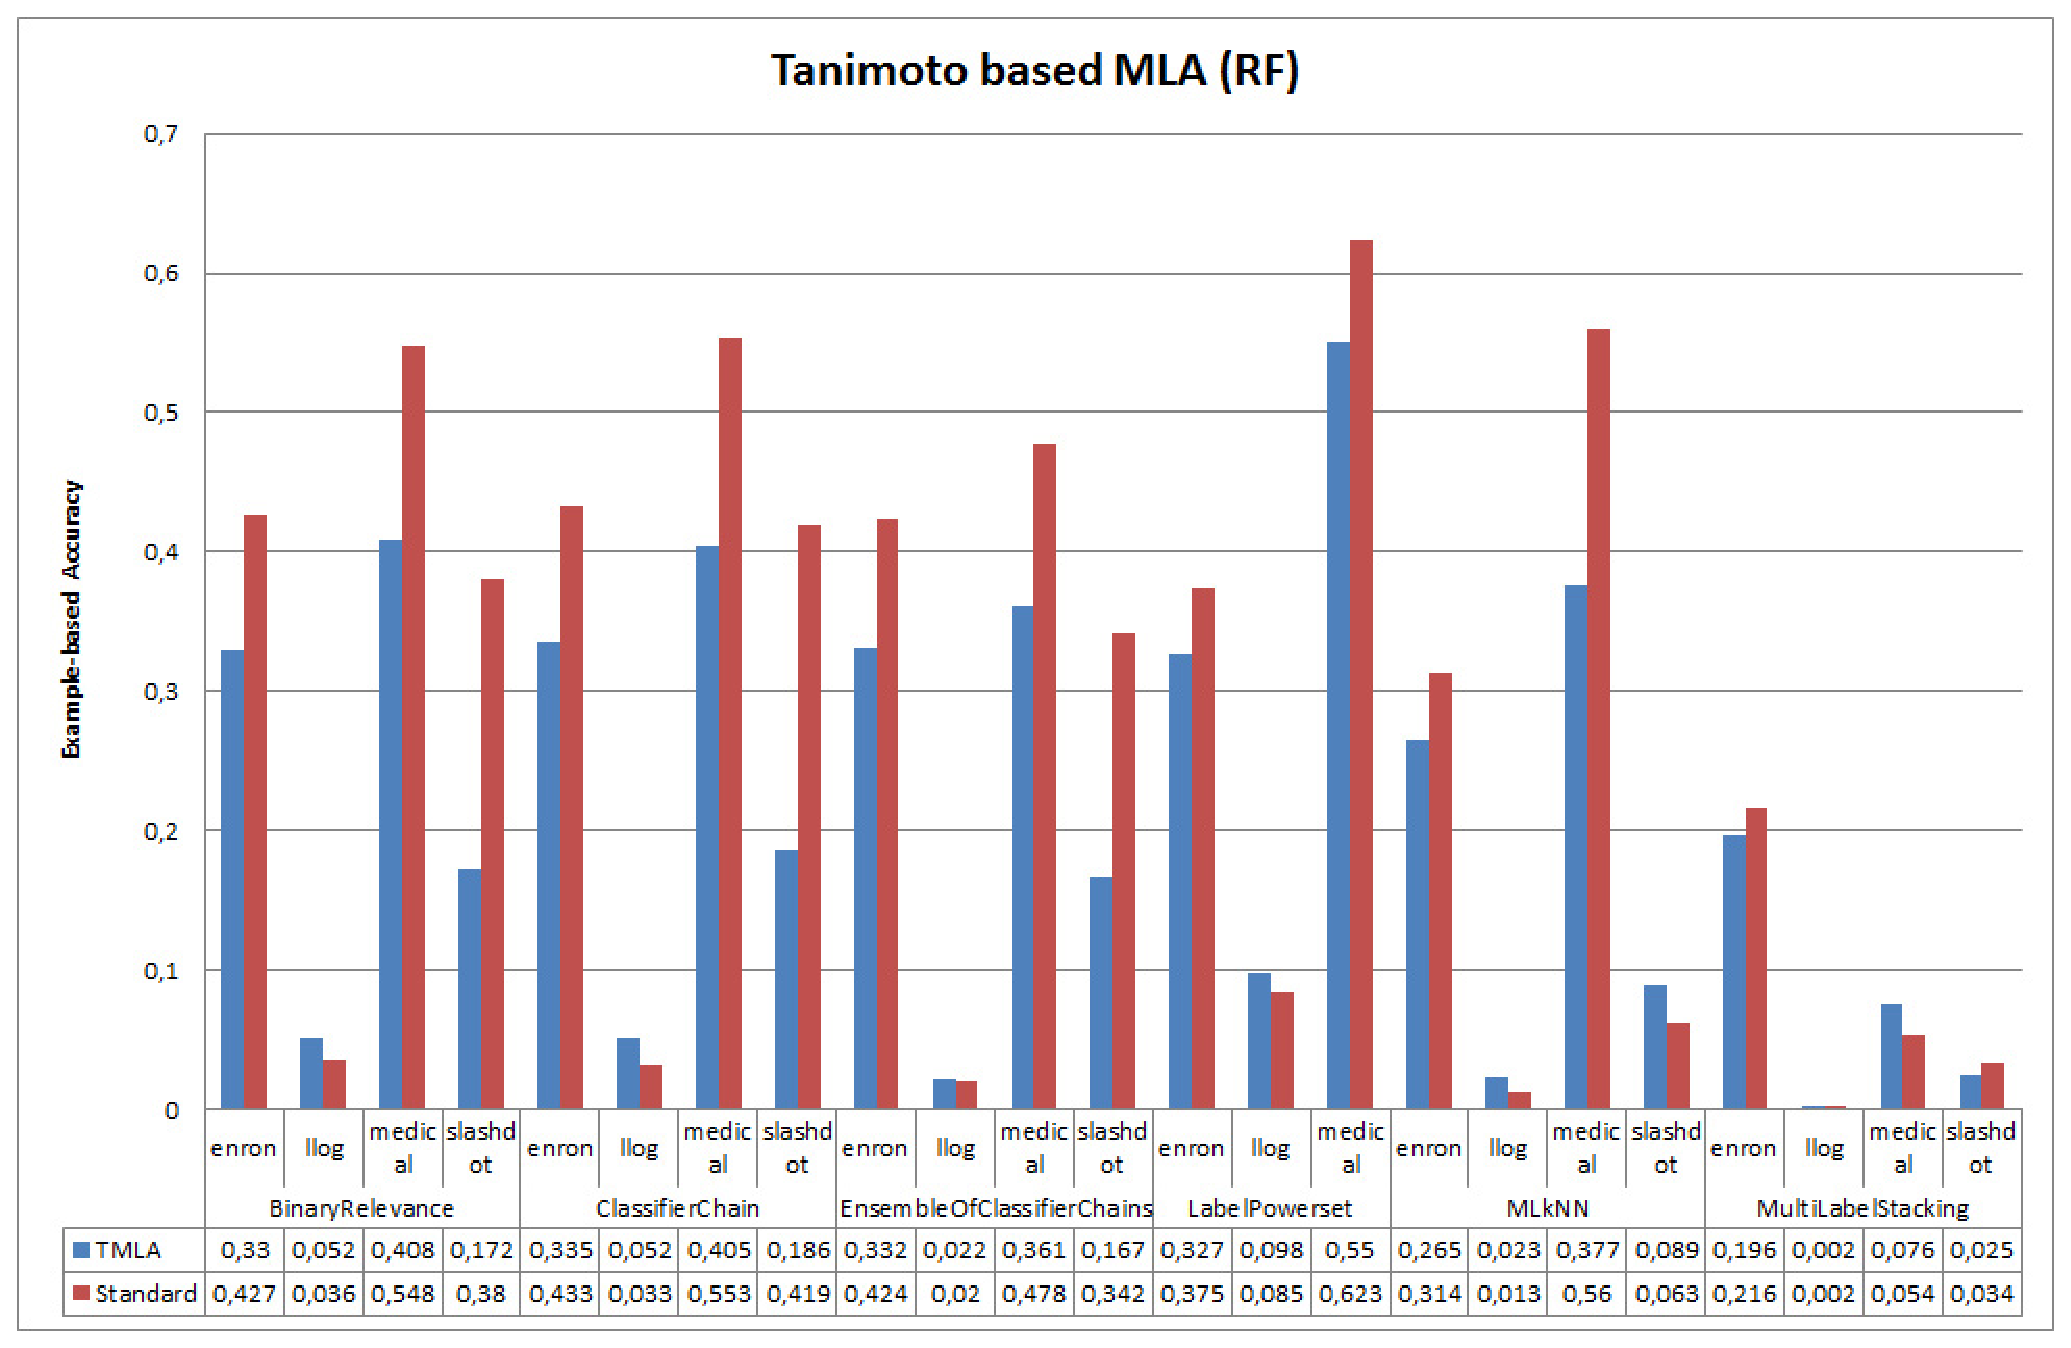
\includegraphics[scale=.3]{figures/tmla_results_rf.eps} 
}

\frame{
	\frametitle{TCML}
	example cluster characteristics (\(\varnothing\) over folds)
	\scriptsize {s
	\begin{itemize}
	  	\item enron\\
		\(\varnothing\) number of clusters : 2\\
		\(\varnothing\) number of clusters ($> 2$ labels) : 2\\
		\(\varnothing\) number of labels per cluster: 31
		\item llog\\
		\(\varnothing\) number of clusters : 2\\
		\(\varnothing\) number of cluster ($> 2$ labels) : 1.8\\
		\(\varnothing\) number of labels per cluster: 40,60	
		\item medical\\
		\(\varnothing\) number of clusters : 6\\
		\(\varnothing\) number of cluster ($> 2$ labels) : 2\\
		\(\varnothing\) number of labels per cluster: 8,9	
		\item slashdot\\
		\(\varnothing\) number of clusters : 2\\
		\(\varnothing\) number of cluster ($> 2$ labels) : 1.8\\
		\(\varnothing\) number of labels per cluster: 14.90	
	\end{itemize}
}
}


\frame{
\frametitle{FCML}
 \begin{itemize} 
  \item feature selection for each label
  \item using log-scores for further processing
  	\begin{eqnarray*} 
      Y_{1} &\leftarrow & \{X_{1}...X_{n} \cup Y_{1}...Y_{n}|X_{i},Y_{i}\in\mathbb R\}\\ 
      &\vdots &\\ 
      Y_{n} &\leftarrow & \{X_{1}...X_{n} \cup Y_{1}...Y_{n}|X_{i},Y_{i}\in\mathbb R\} 
    \end{eqnarray*} 
  	\item Hierachical Clustering using Chebyshev-, Euclidean-, Manhatten-, Mikowski-Distance
  	\item Single, Complete, Average and Mean Clustering
  	\item no. of clusters: $2,4,6$
  	 \end{itemize}
}

%\frame{
% {\insertsection} 
% \begin{itemize} 
%  \item \begin{scriptsize}
%		\begin{algorithmic}
%		   \Function{findLabelFeatureSets}{clusters}
%			   	\State $ groups \gets Map<labelSet, featureSet> $
%		   		\For{$ C \in clusters $} \Comment{every cluster}
%		   			\State $currentLabelSet, currentFeatureSet $
%		   			\For{ $ I \in C $ } \Comment{every instance}
%						\For{ $ A \in I $ } \Comment{every attribute}
%							\If{ $ score(A) > threshold $ }
%								\If{ $ A \in labelSet $ }
%									\State $ currentLabelSet \cap \{A\} $
%								\Else
%									\State $ currentFeatureSet \cap \{A\} $
%								\EndIf
%							\EndIf
%		    			\EndFor
%		    		\EndFor
%		    		\State $ put(currentLabelSet, currentFeatureSet) \rightarrow groups $
%		    	\EndFor
%		    	\Return $groups$
%		    \EndFunction
%		  \end{algorithmic}
%		\end{scriptsize}
%	\end{itemize}
%}

\frame{
 {\insertsection} 
		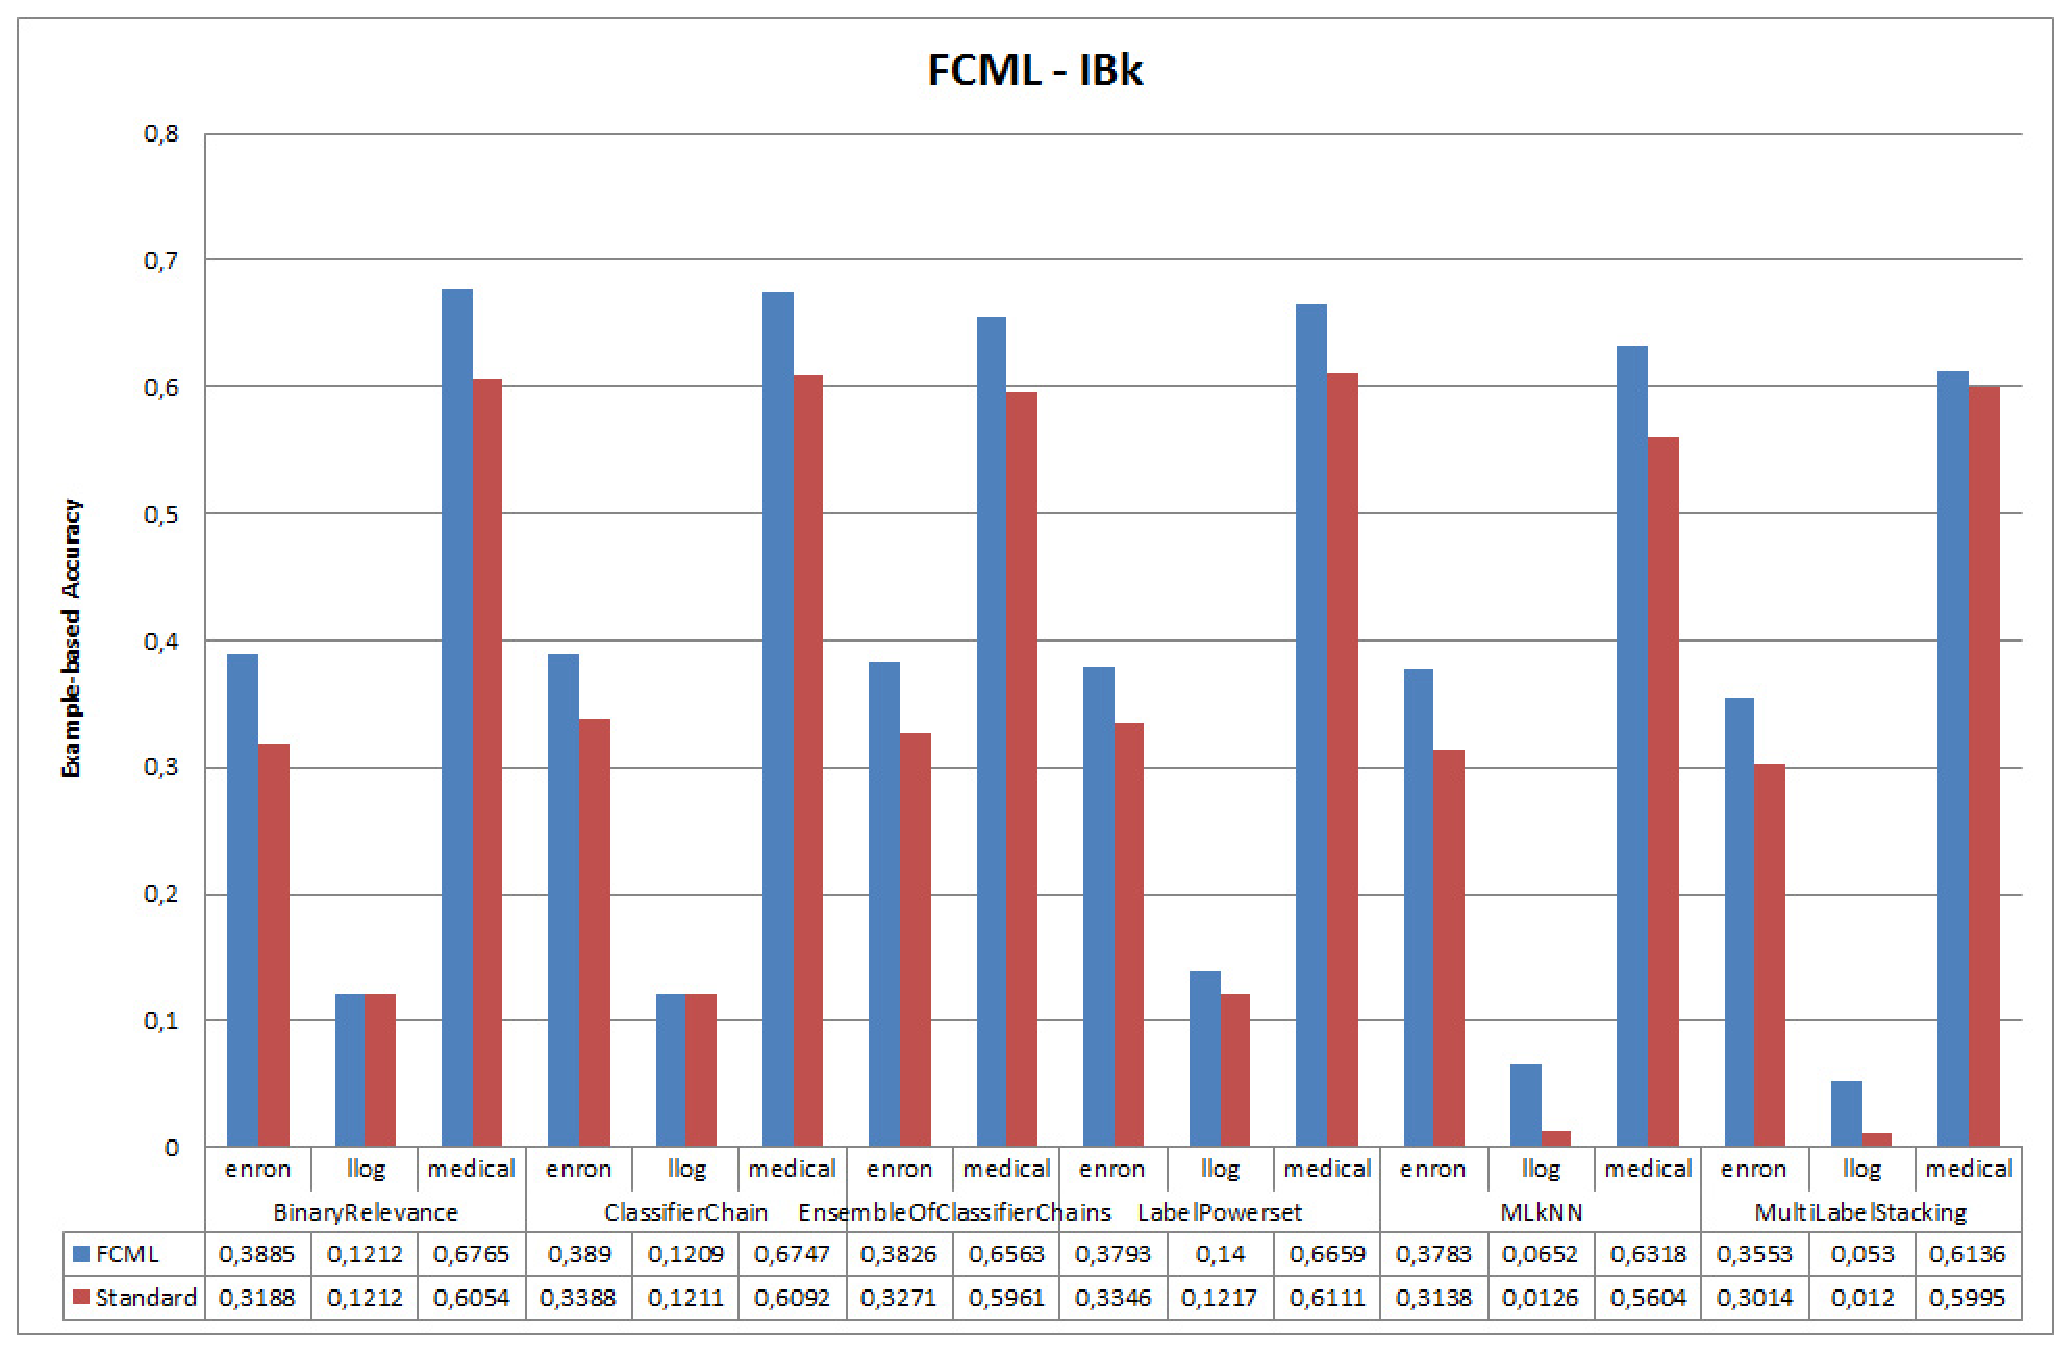
\includegraphics[scale=.3]{figures/fcml_results_ibk.eps} 
}


\frame{
 {\insertsection} 
		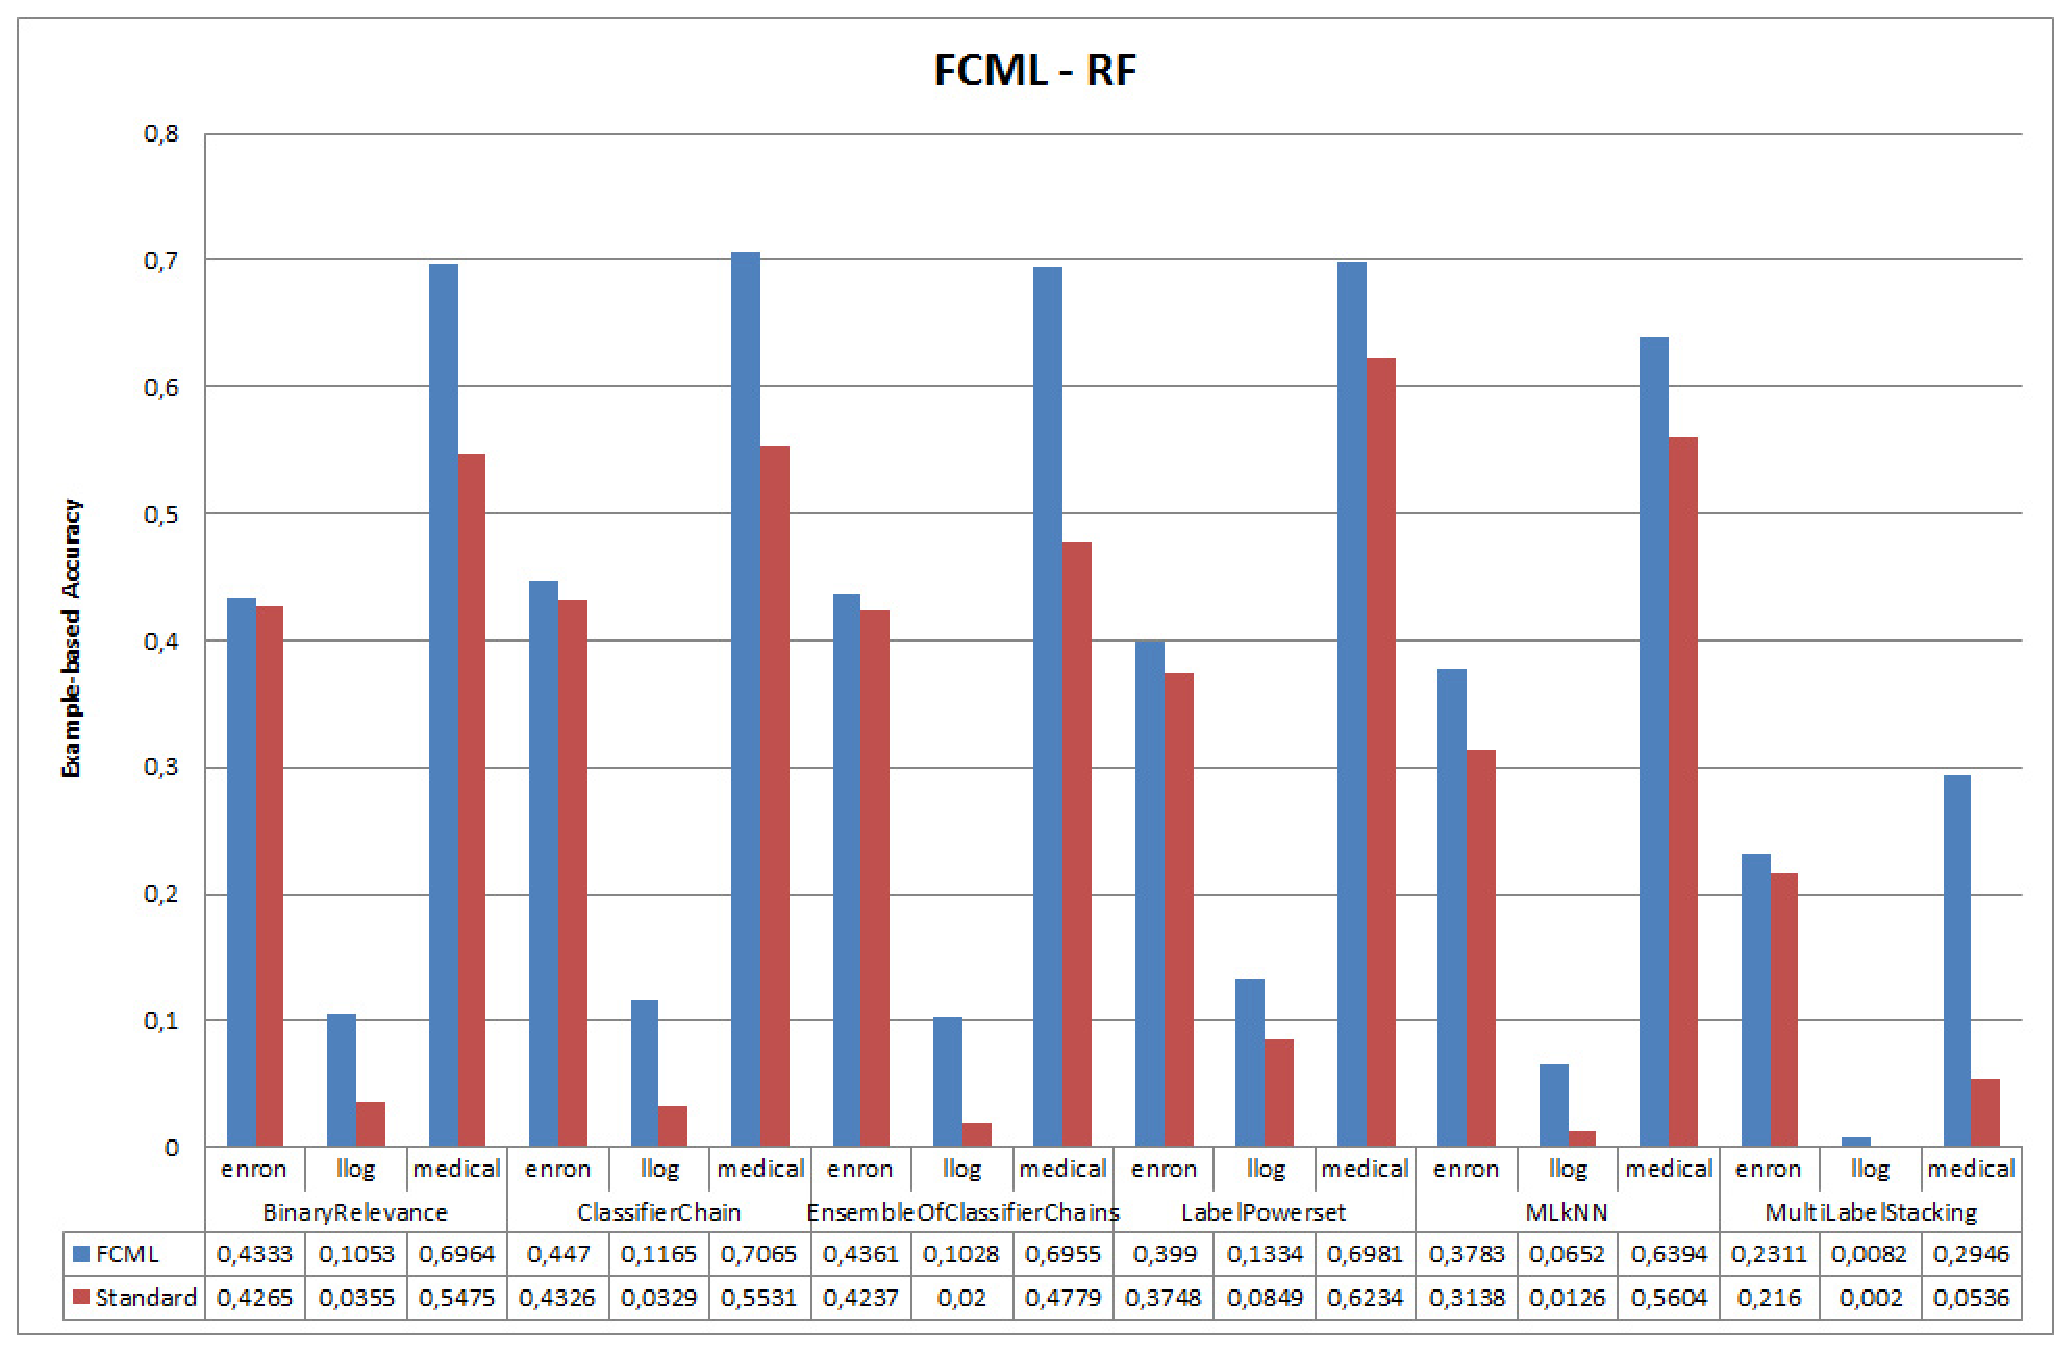
\includegraphics[scale=.3]{figures/fcml_results_rf.eps} 
}


\frame{
 {\insertsection} 
		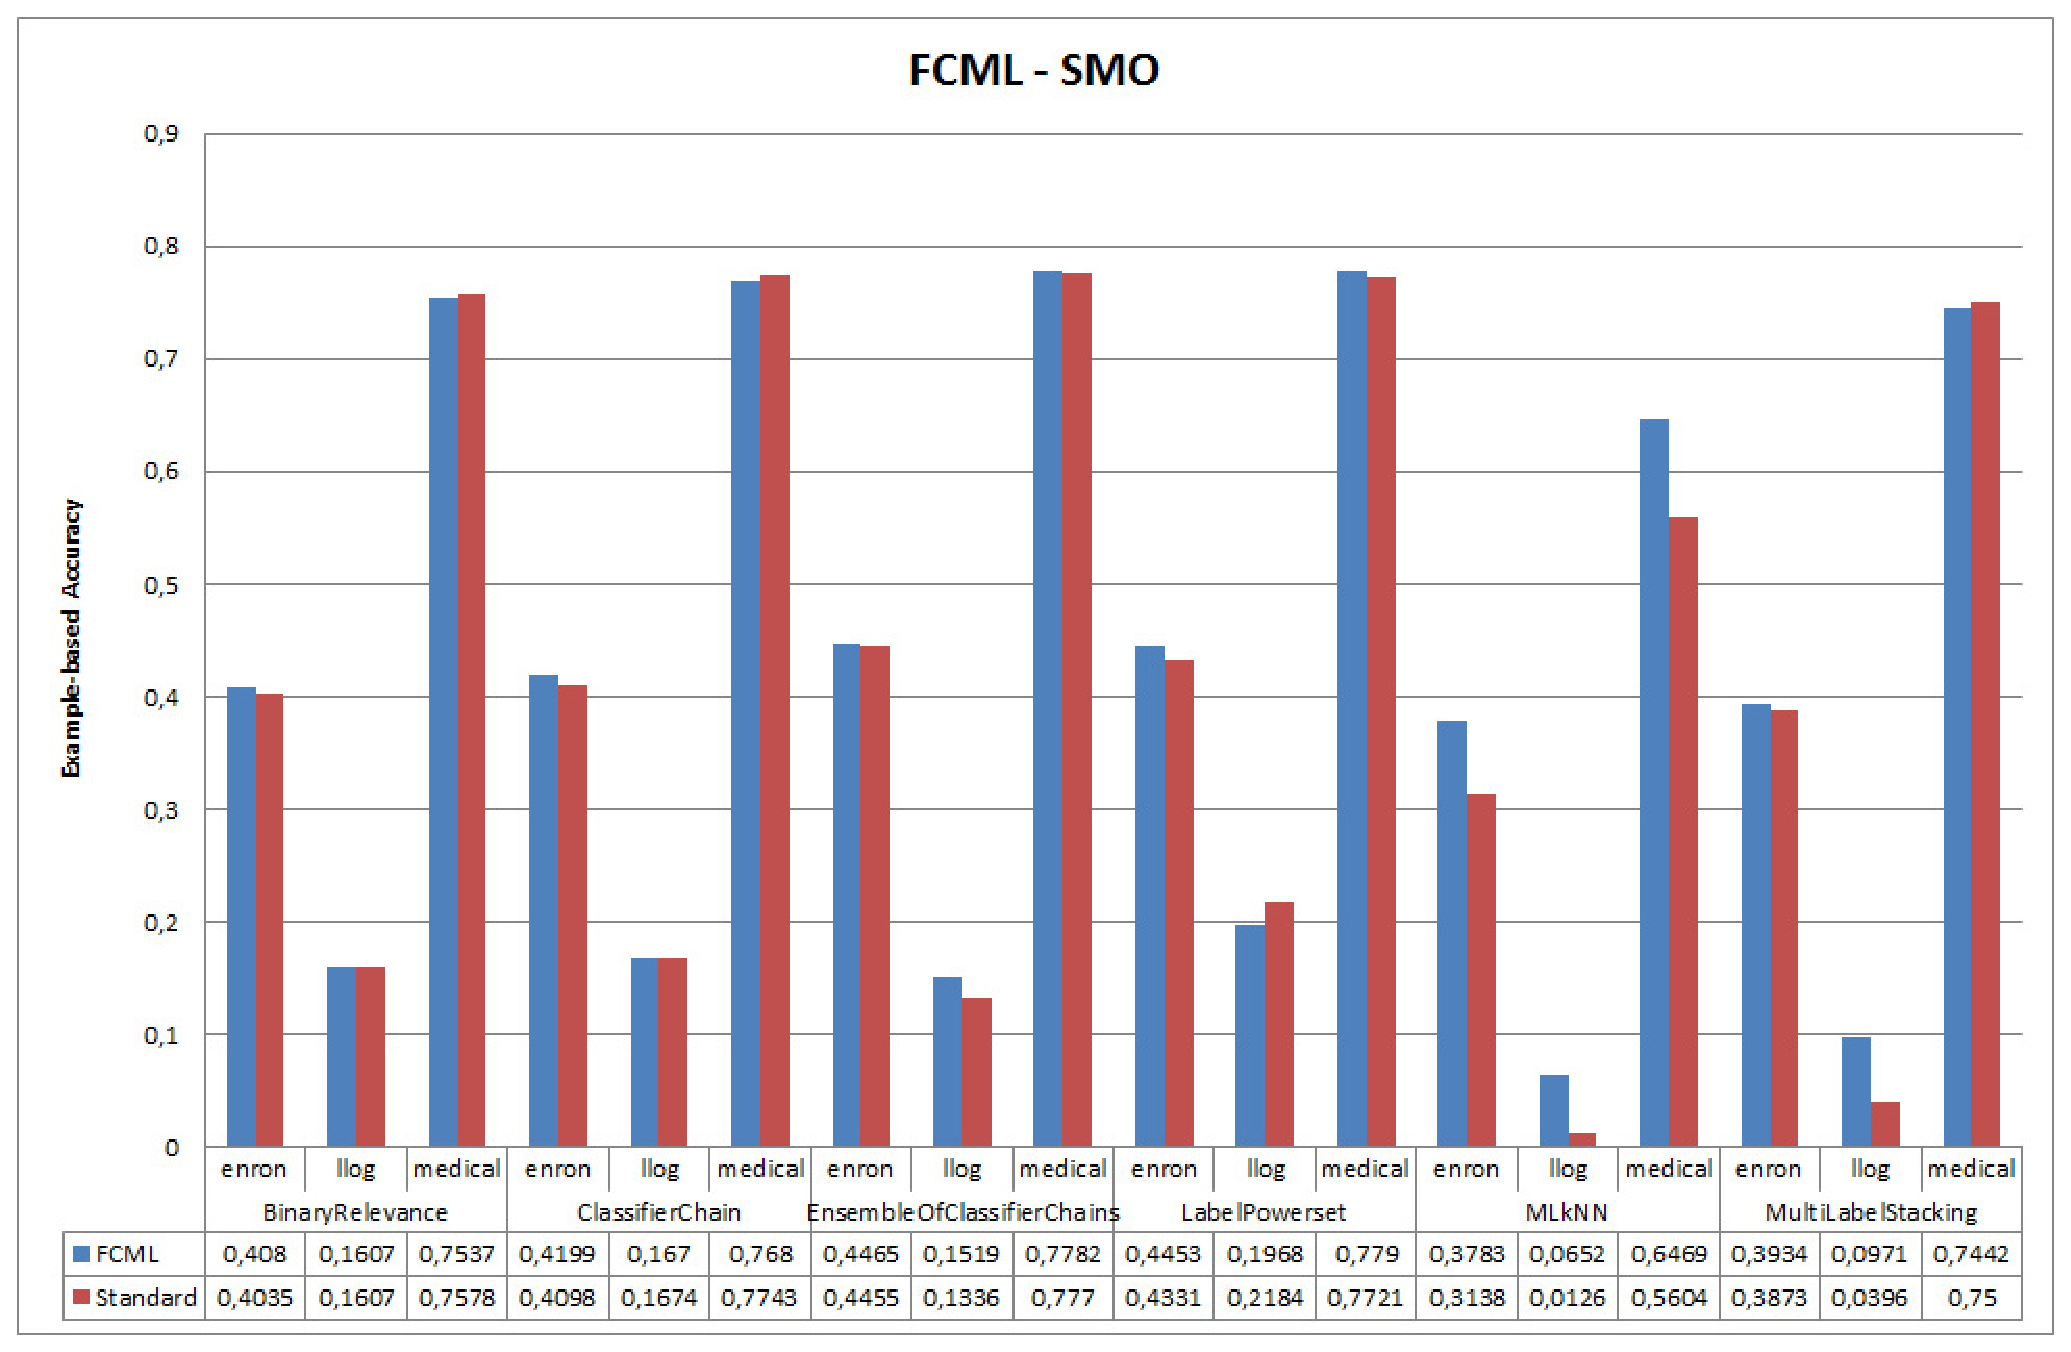
\includegraphics[scale=.3]{figures/fcml_results_smo.eps} 
}

\frame{
\frametitle{FCML}
	example cluster characteristics (\(\varnothing\) over folds)
	\scriptsize {
	\begin{itemize}
		\item enron\\
		\(\varnothing\) number of clusters : 2\\
		\(\varnothing\) number of cluster ($> 2$ labels) : 2\\
		\(\varnothing\) number of labels per cluster: 26.5
		\item llog\\
		\(\varnothing\) number of clusters : 2 \\
		\(\varnothing\) number of cluster ($> 2$ labels) : 2\\
		\(\varnothing\) number of labels per cluster: 37.5	
		\item medical\\
		\(\varnothing\) number of clusters : 4\\
		\(\varnothing\) number of cluster ($> 2$ labels) : 1\\
		\(\varnothing\) number of labels per cluster: 11.25
	\end{itemize}
	}
}

\frame{
	\frametitle{Future Work}
	\begin{itemize}
		\item use ranking instead of scores (Spearman Correlation)
		\item remove outliers to reduce noice and find better groups (covering at least $ 10\% $ of all labels)
	\end{itemize}		
}

\end{document}